\documentclass{ctexart}

\title{基于彩色 CCD 的棱镜摄谱实验\\{\large 实验报告}}
\author{\Large  PB22051031 李毅\\{\large PHYS1009B.02 }\\{教室:一教1321\quad 座位号:5}}
\date{\today}
\usepackage{amsmath}
\usepackage{amsfonts}
\usepackage{amssymb}
\usepackage{bm}
\usepackage{enumerate}
\usepackage{geometry}
\geometry{left=3.0cm,right=3.0cm,top=2.5cm,bottom=2.5cm}
\usepackage{fancyhdr}
\pagestyle{fancy}
\fancyhead[l]{ }
\fancyhead[r]{ }
\fancyhead[C]{
	\begin{tabular}{cccc}
		&\multicolumn{2}{c}\large{\textbf{中国科学技术大学物理实验报告}}\\
		\vspace{0.1cm}信息科学技术学院 & PB22051031\ 李毅 & PHYS1009B.02 & \today 
\end{tabular}}
\fancyfoot[C]{ 第 {\thepage} 页,共 \pageref{unknown} 页}
\renewcommand{\headrulewidth}{2pt}
\usepackage{graphicx}
\usepackage{geometry}
\usepackage[hidelinks]{hyperref}
\usepackage{multicol}
\usepackage{multirow}
\usepackage{ragged2e}
\usepackage[square,comma,numbers,super]{natbib}
\bibliographystyle{unsrt}
\usepackage{siunitx}
\usepackage{subfigure}
\usepackage{wrapfig}
\usepackage{xcolor}
\usepackage{cite}
\begin{document}
	\maketitle
    \newpage
    \section*{第一部分\quad 实验原理}
    棱镜摄谱仪是利用棱镜作为分光元件的摄谱仪器。本次实验所用的是可见光范围内的小型棱镜摄谱仪,如图1所示。$S$ 为光源, $L$ 为聚光透镜,使 $S$ 发出的发散光会聚后均匀照亮狭缝,$S_1$为狭缝,以控制入射光的宽度; $L_1$ 为准直透镜,和 $S_1$ 的距离大小等于其焦距,产生平行光后, 均匀的照射在阿贝棱镜的入射面上,这是摄谱仪的第一部分。 
    
    经透镜 $L_1$ 照射过来的平行光,通过阿贝复合棱镜分光转向出射,此时各种单色光不再相互平行,而是之间有相互较小的夹角。至此完成了摄谱仪的第二部分。

    经过分光后的各种单色光,由会聚透镜 $L_2$,将各种分离的单色光会聚成单一谱线, 成像于 $L_2$ 的谱平面上。将彩色 $CCD$ 的成像面置于 $L_2$ 的谱平面上; 通过彩色 $CCD$ 连接到计算机和显示器,可以看到各种分离的彩色谱线,并记录成图片格式存储。由于氦谱在可见光范围内谱线相对较多,一般用来作为已知光谱。接着计算机对这些图片进行比对,用插值法,从已知谱线和未知谱线的位置(像素) 关系上,就可以计算出未知谱线。
    
    插值法的原理如下:设未知谱线像素位置为$d_x$,2条已知谱线位置分别为$d_1$,$d_2$,波长分别为$\lambda_1$,$\lambda_2$。则未知谱线的波长$\lambda_x$由线性插值公式
    $$\lambda_x=\lambda_1+(\lambda_2-\lambda_1)\dfrac{d_x-d_1}{d_2-d_1}$$
给出。


    \begin{minipage}[l]{1\textwidth}
        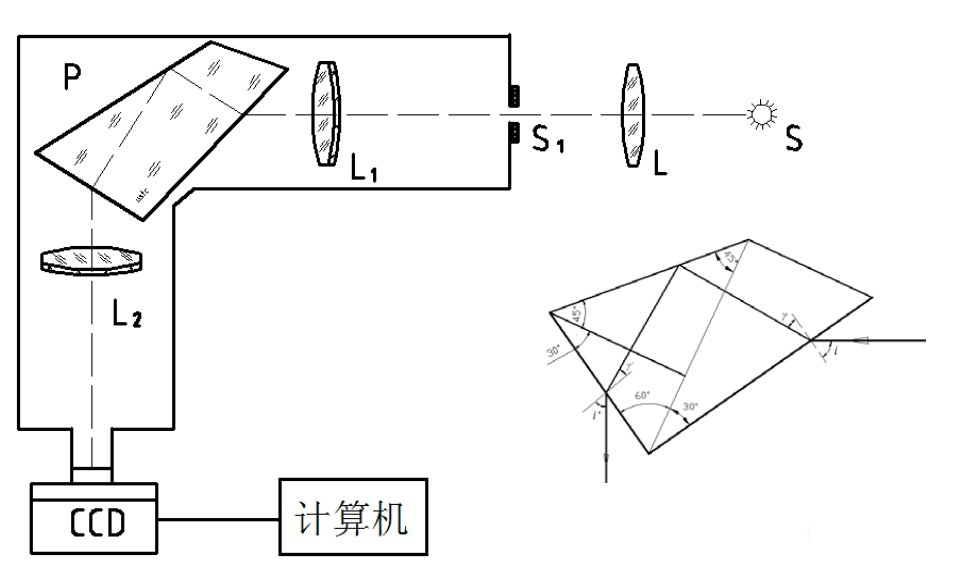
\includegraphics[scale=1.2]{1} \\\small{图1.棱镜摄谱仪原理简图和阿贝复合棱镜截面图}\centering
    \end{minipage}
    \newpage
    \section*{第二部分 \qquad 实验步骤与数据处理}
    将氦灯光源置于光路中观察谱线。调节光源、会聚透镜 L、狭缝中心处于等高共轴状态,使用目镜观察谱线,并通过调节会聚透镜 $L_2$ 的调节旋钮,使用目镜观察谱线直到清晰为止。接着使用CCD进行摄谱。

    实验使用1/2英寸的CCD,光谱线宽度比 CCD 靶面要宽,所以整个光谱线要用三张图片分段拍摄,处理时将三幅图片拼接在一起成为一个整体。先拍摄氦灯光源可见光长波段(红、黄) 的光谱谱线图片,调整谱线亮度、粗细合适后,拍摄 1 次。保持 CCD 位置不动,换上汞灯光源并调整,拍摄 1 次。再换上钠灯光源并调整,拍摄 1 次。拍摄完图像后,按照具体拍摄的光源谱线对图像进行命名保存。移动 CCD 至光谱的中间位置,重复上述过程;移动 CCD 至光谱的右边位置,重复上述过程。得到以下9张图片:

~\\
\begin{minipage}[c]{0.33\textwidth}
    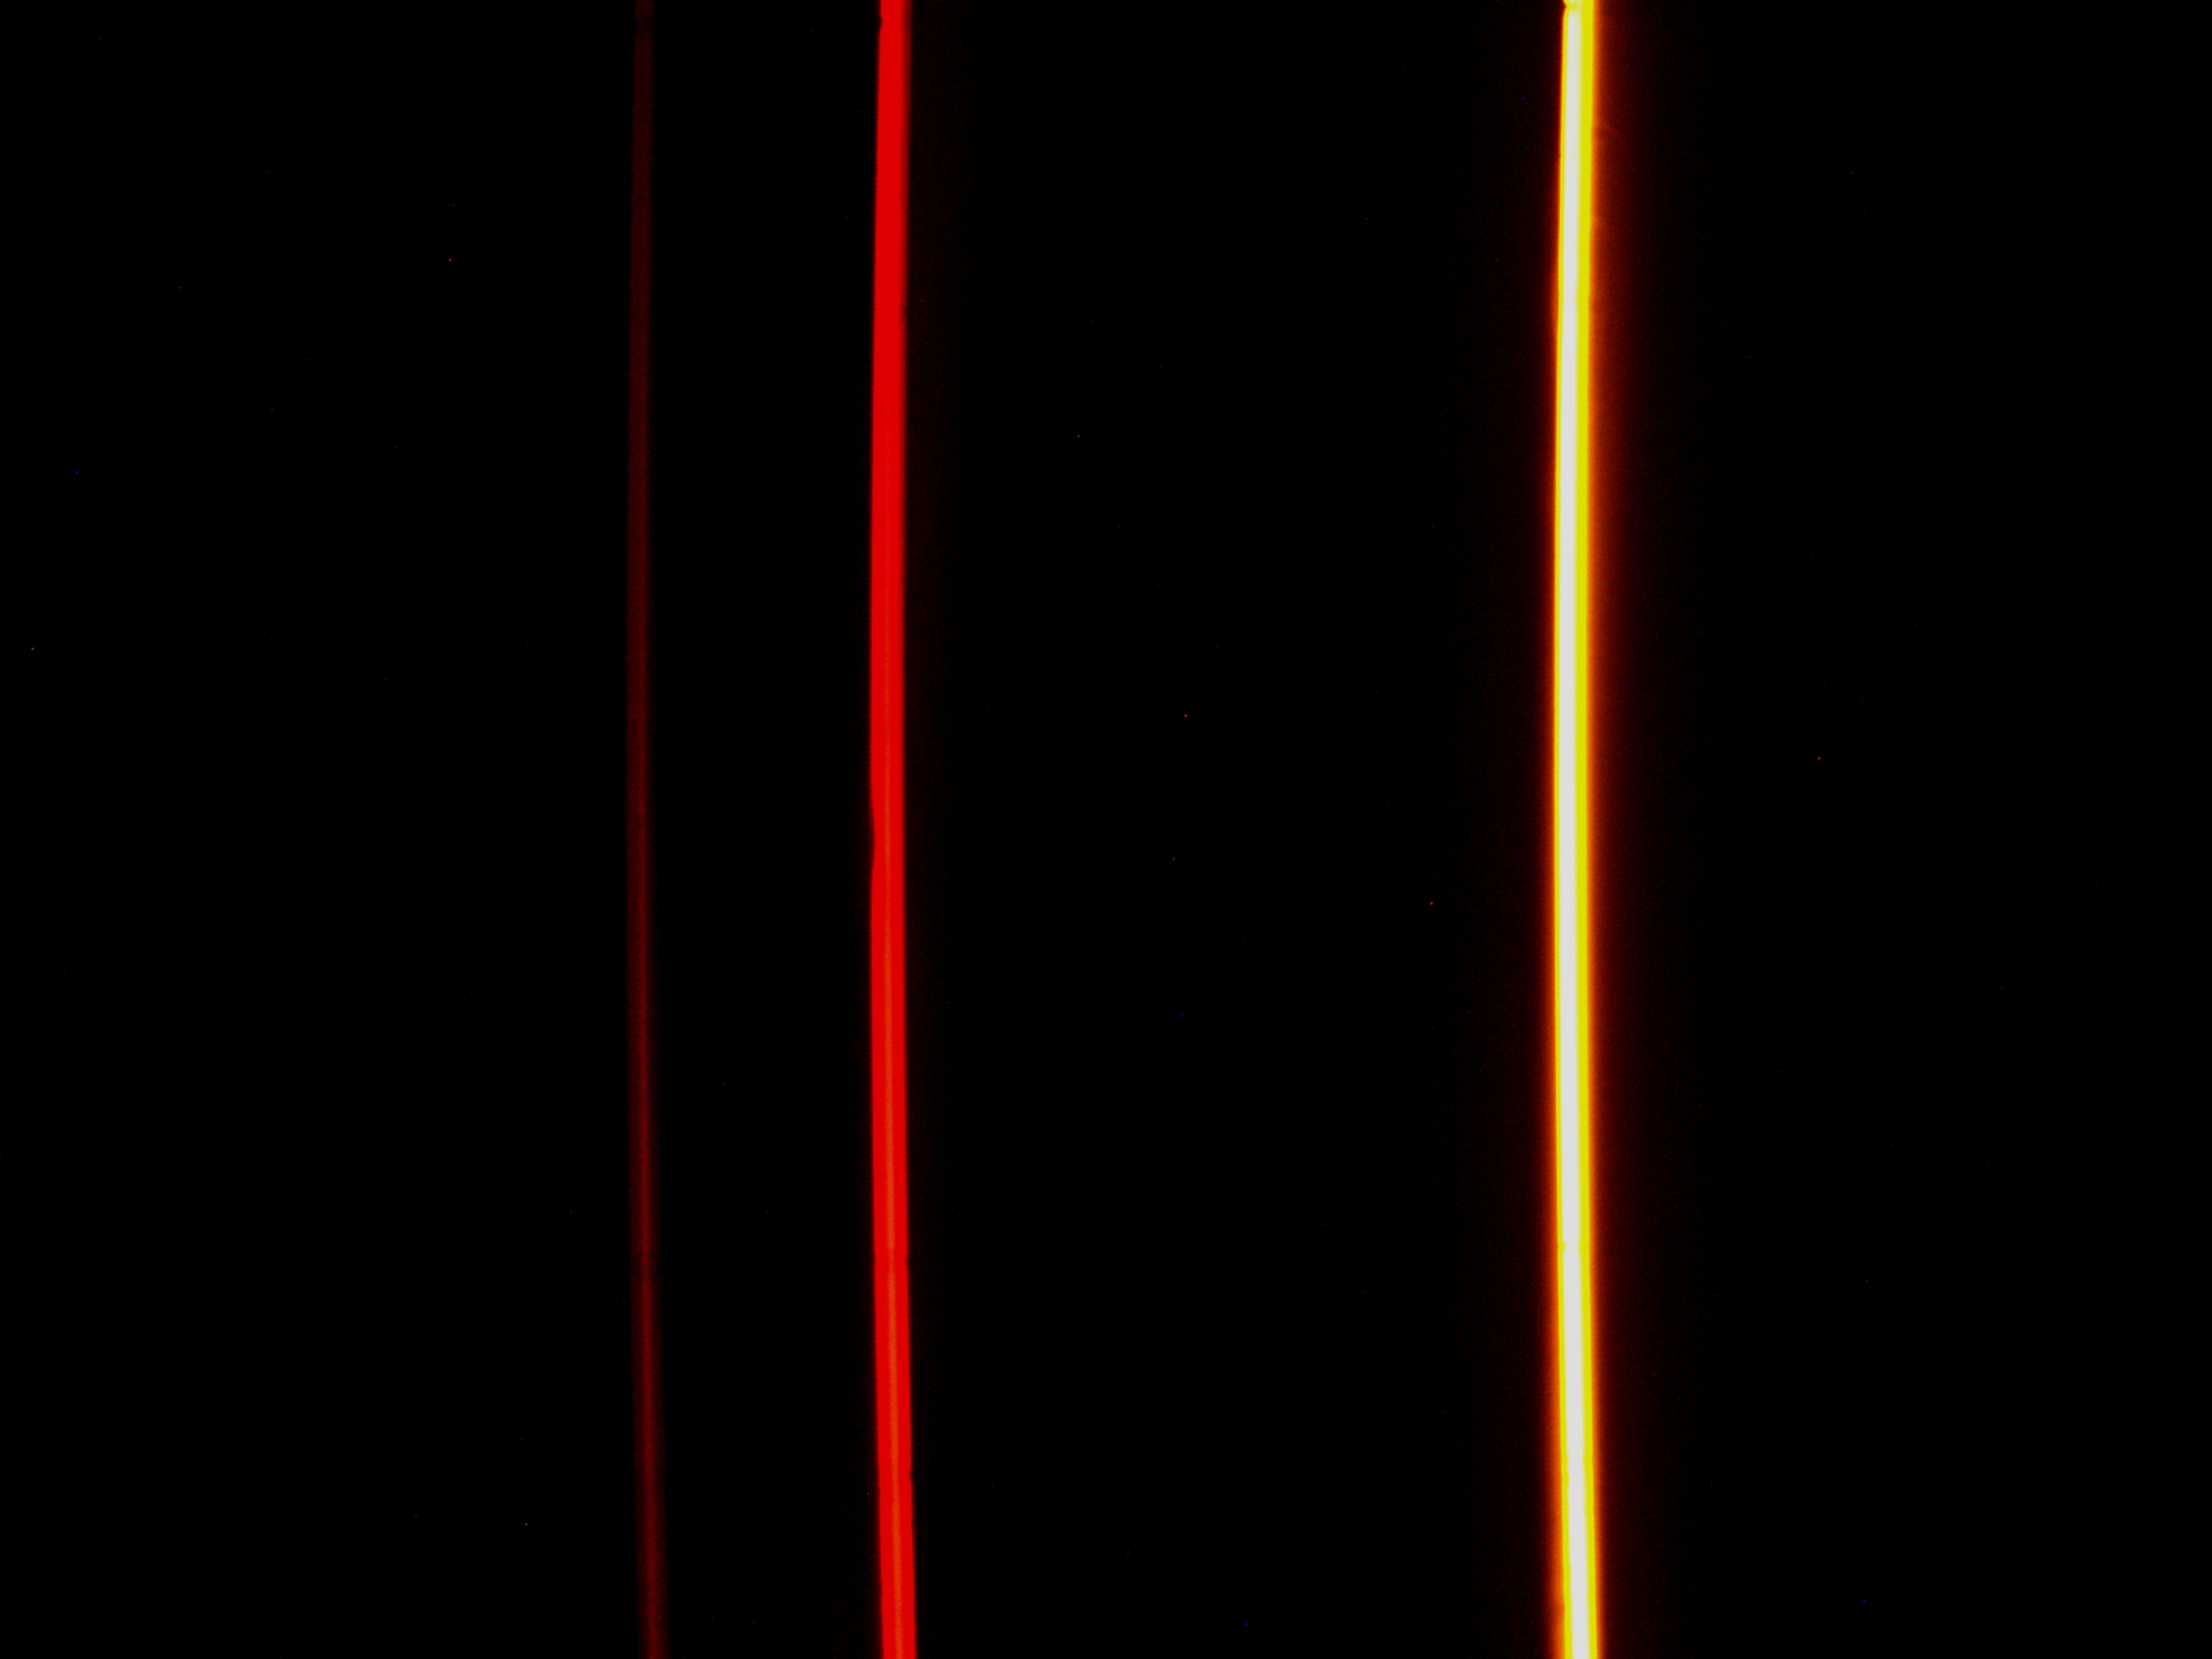
\includegraphics[scale=0.05]{1-1} \\\small{图2.1.1 氦灯左边位置}\centering
\end{minipage}
\begin{minipage}[c]{0.33\textwidth}
    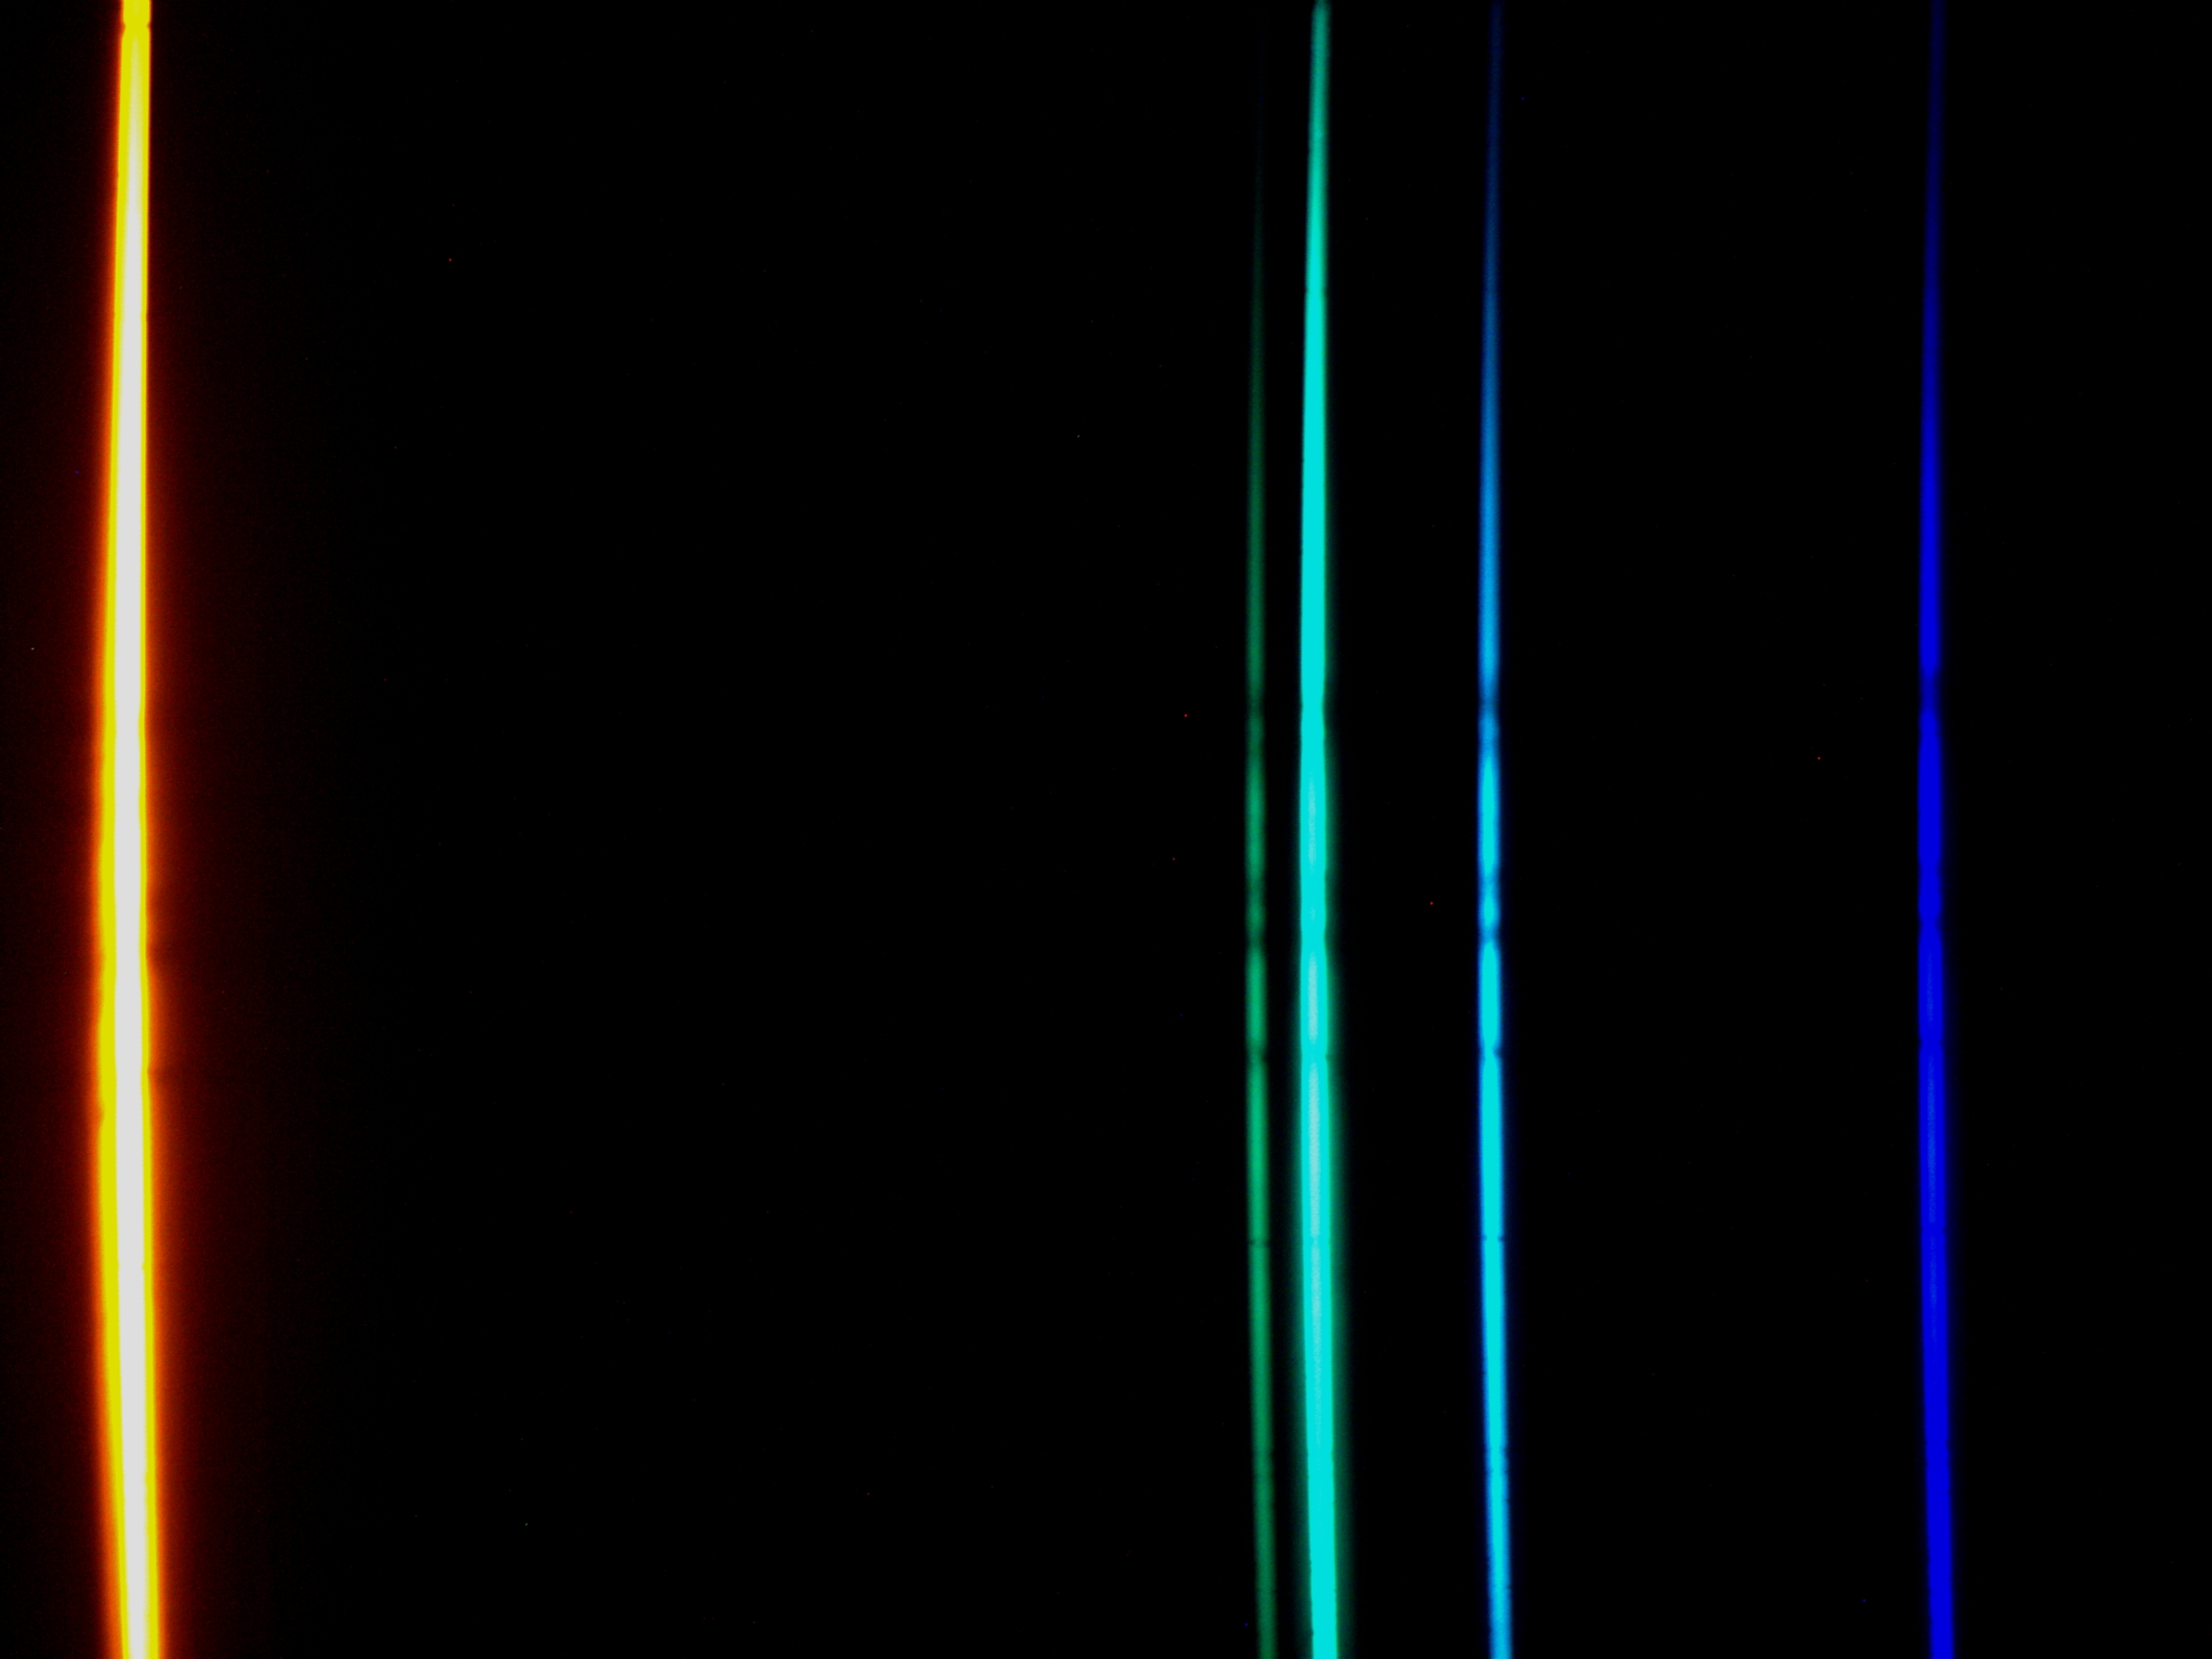
\includegraphics[scale=0.05]{2-1} \\\small{图2.1.2 氦灯中间位置}\centering
\end{minipage}
\begin{minipage}[c]{0.33\textwidth}
    
\includegraphics[scale=0.05]{3-1} \\\small{图2.1.3 氦灯右边位置}\centering
\end{minipage}

~\\
\begin{minipage}[c]{0.33\textwidth}
    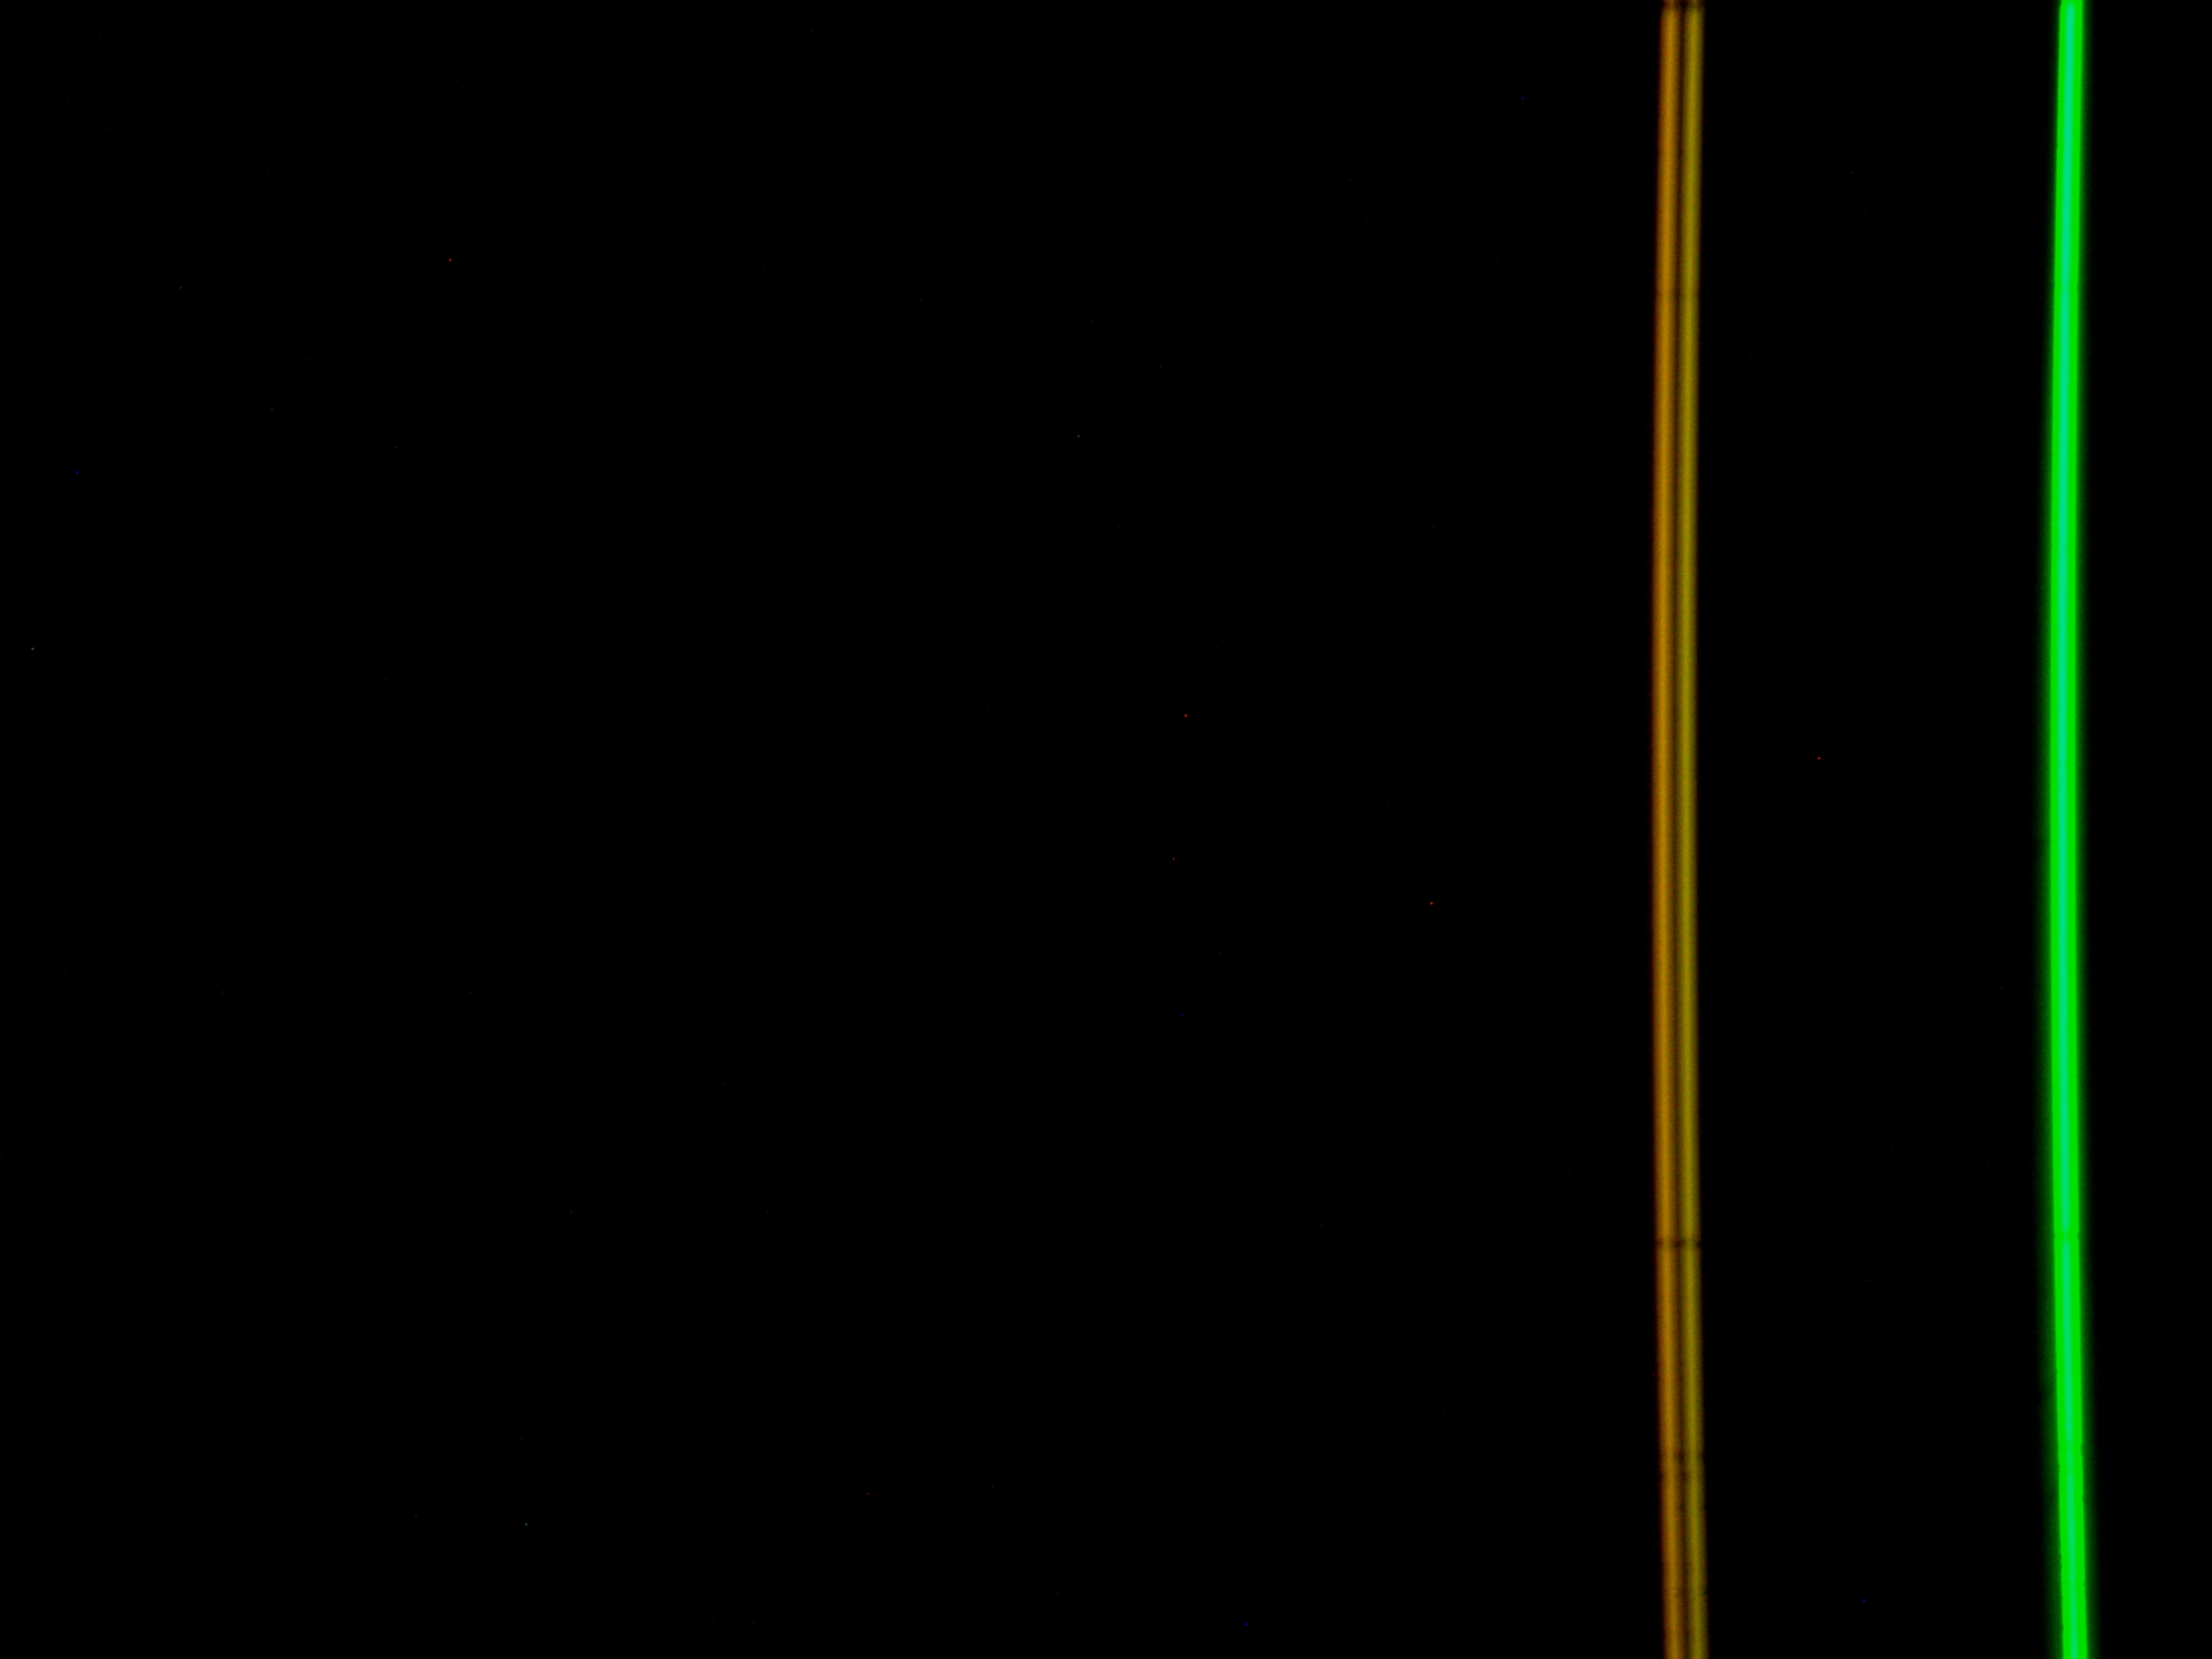
\includegraphics[scale=0.05]{1-2} \\\small{图2.2.1 汞灯左边位置}\centering
\end{minipage}
\begin{minipage}[c]{0.33\textwidth}
    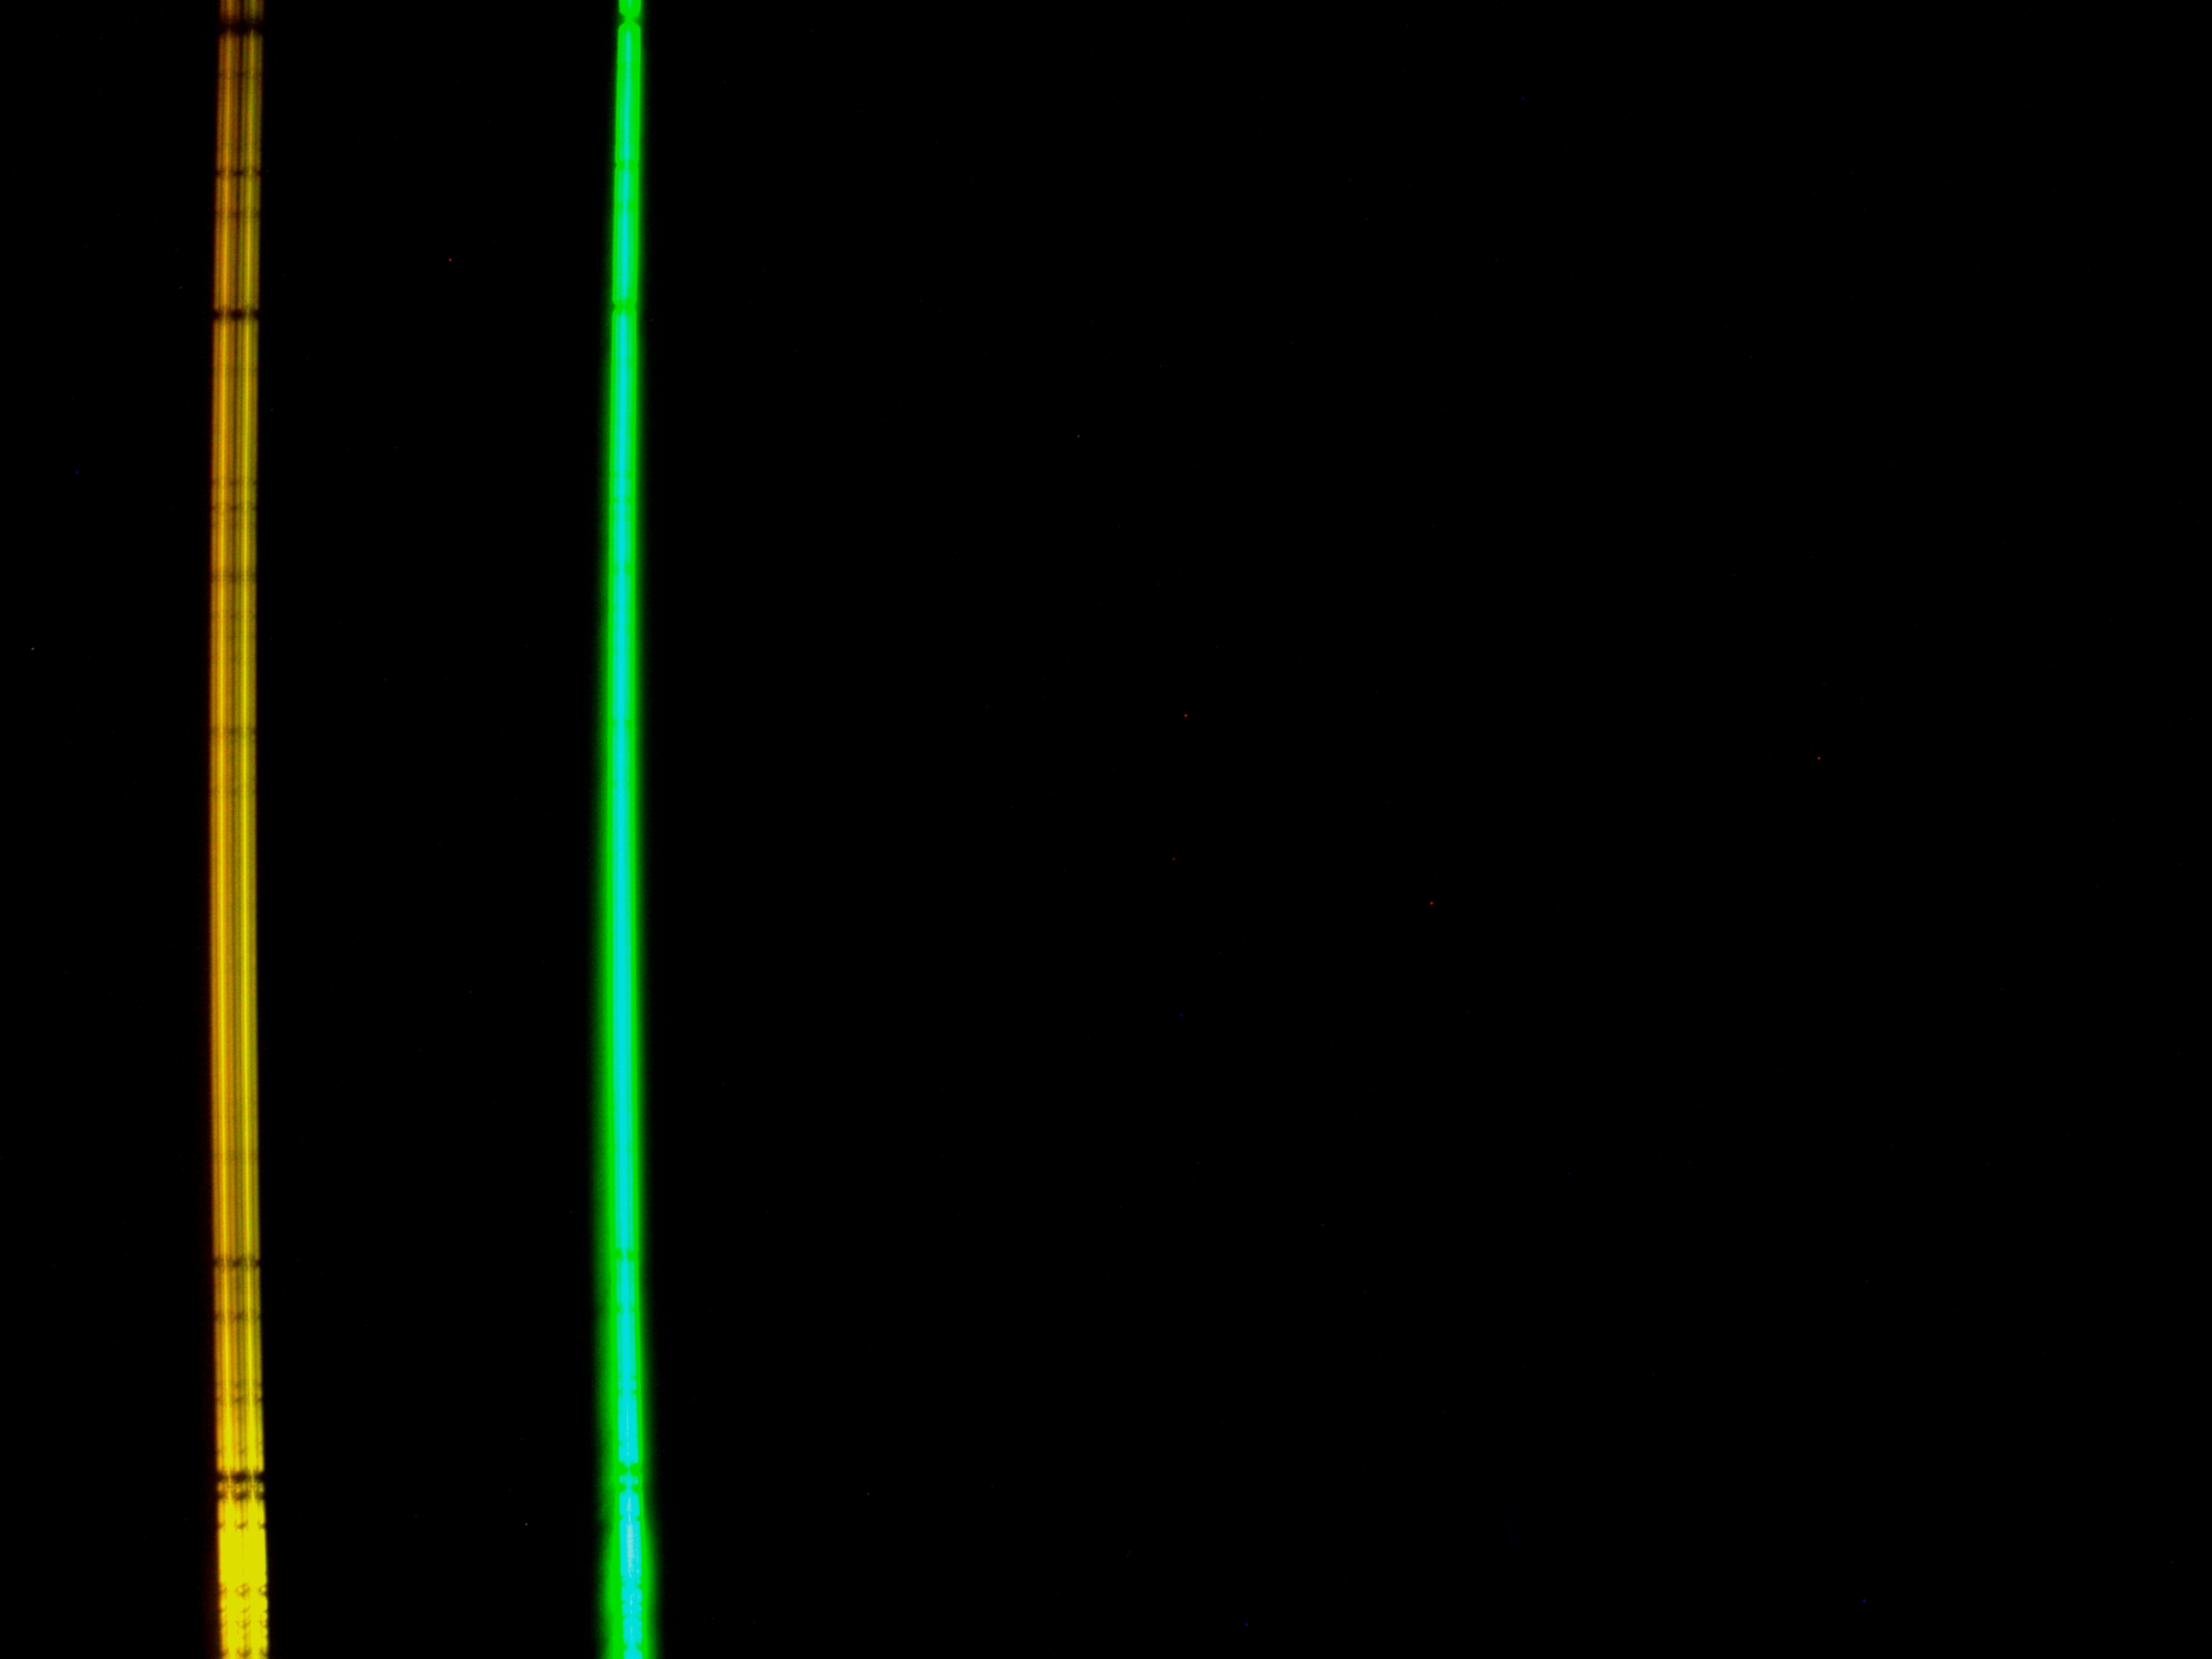
\includegraphics[scale=0.05]{2-2} \\\small{图2.2.2 汞灯中间位置}\centering
\end{minipage}
\begin{minipage}[c]{0.33\textwidth}
    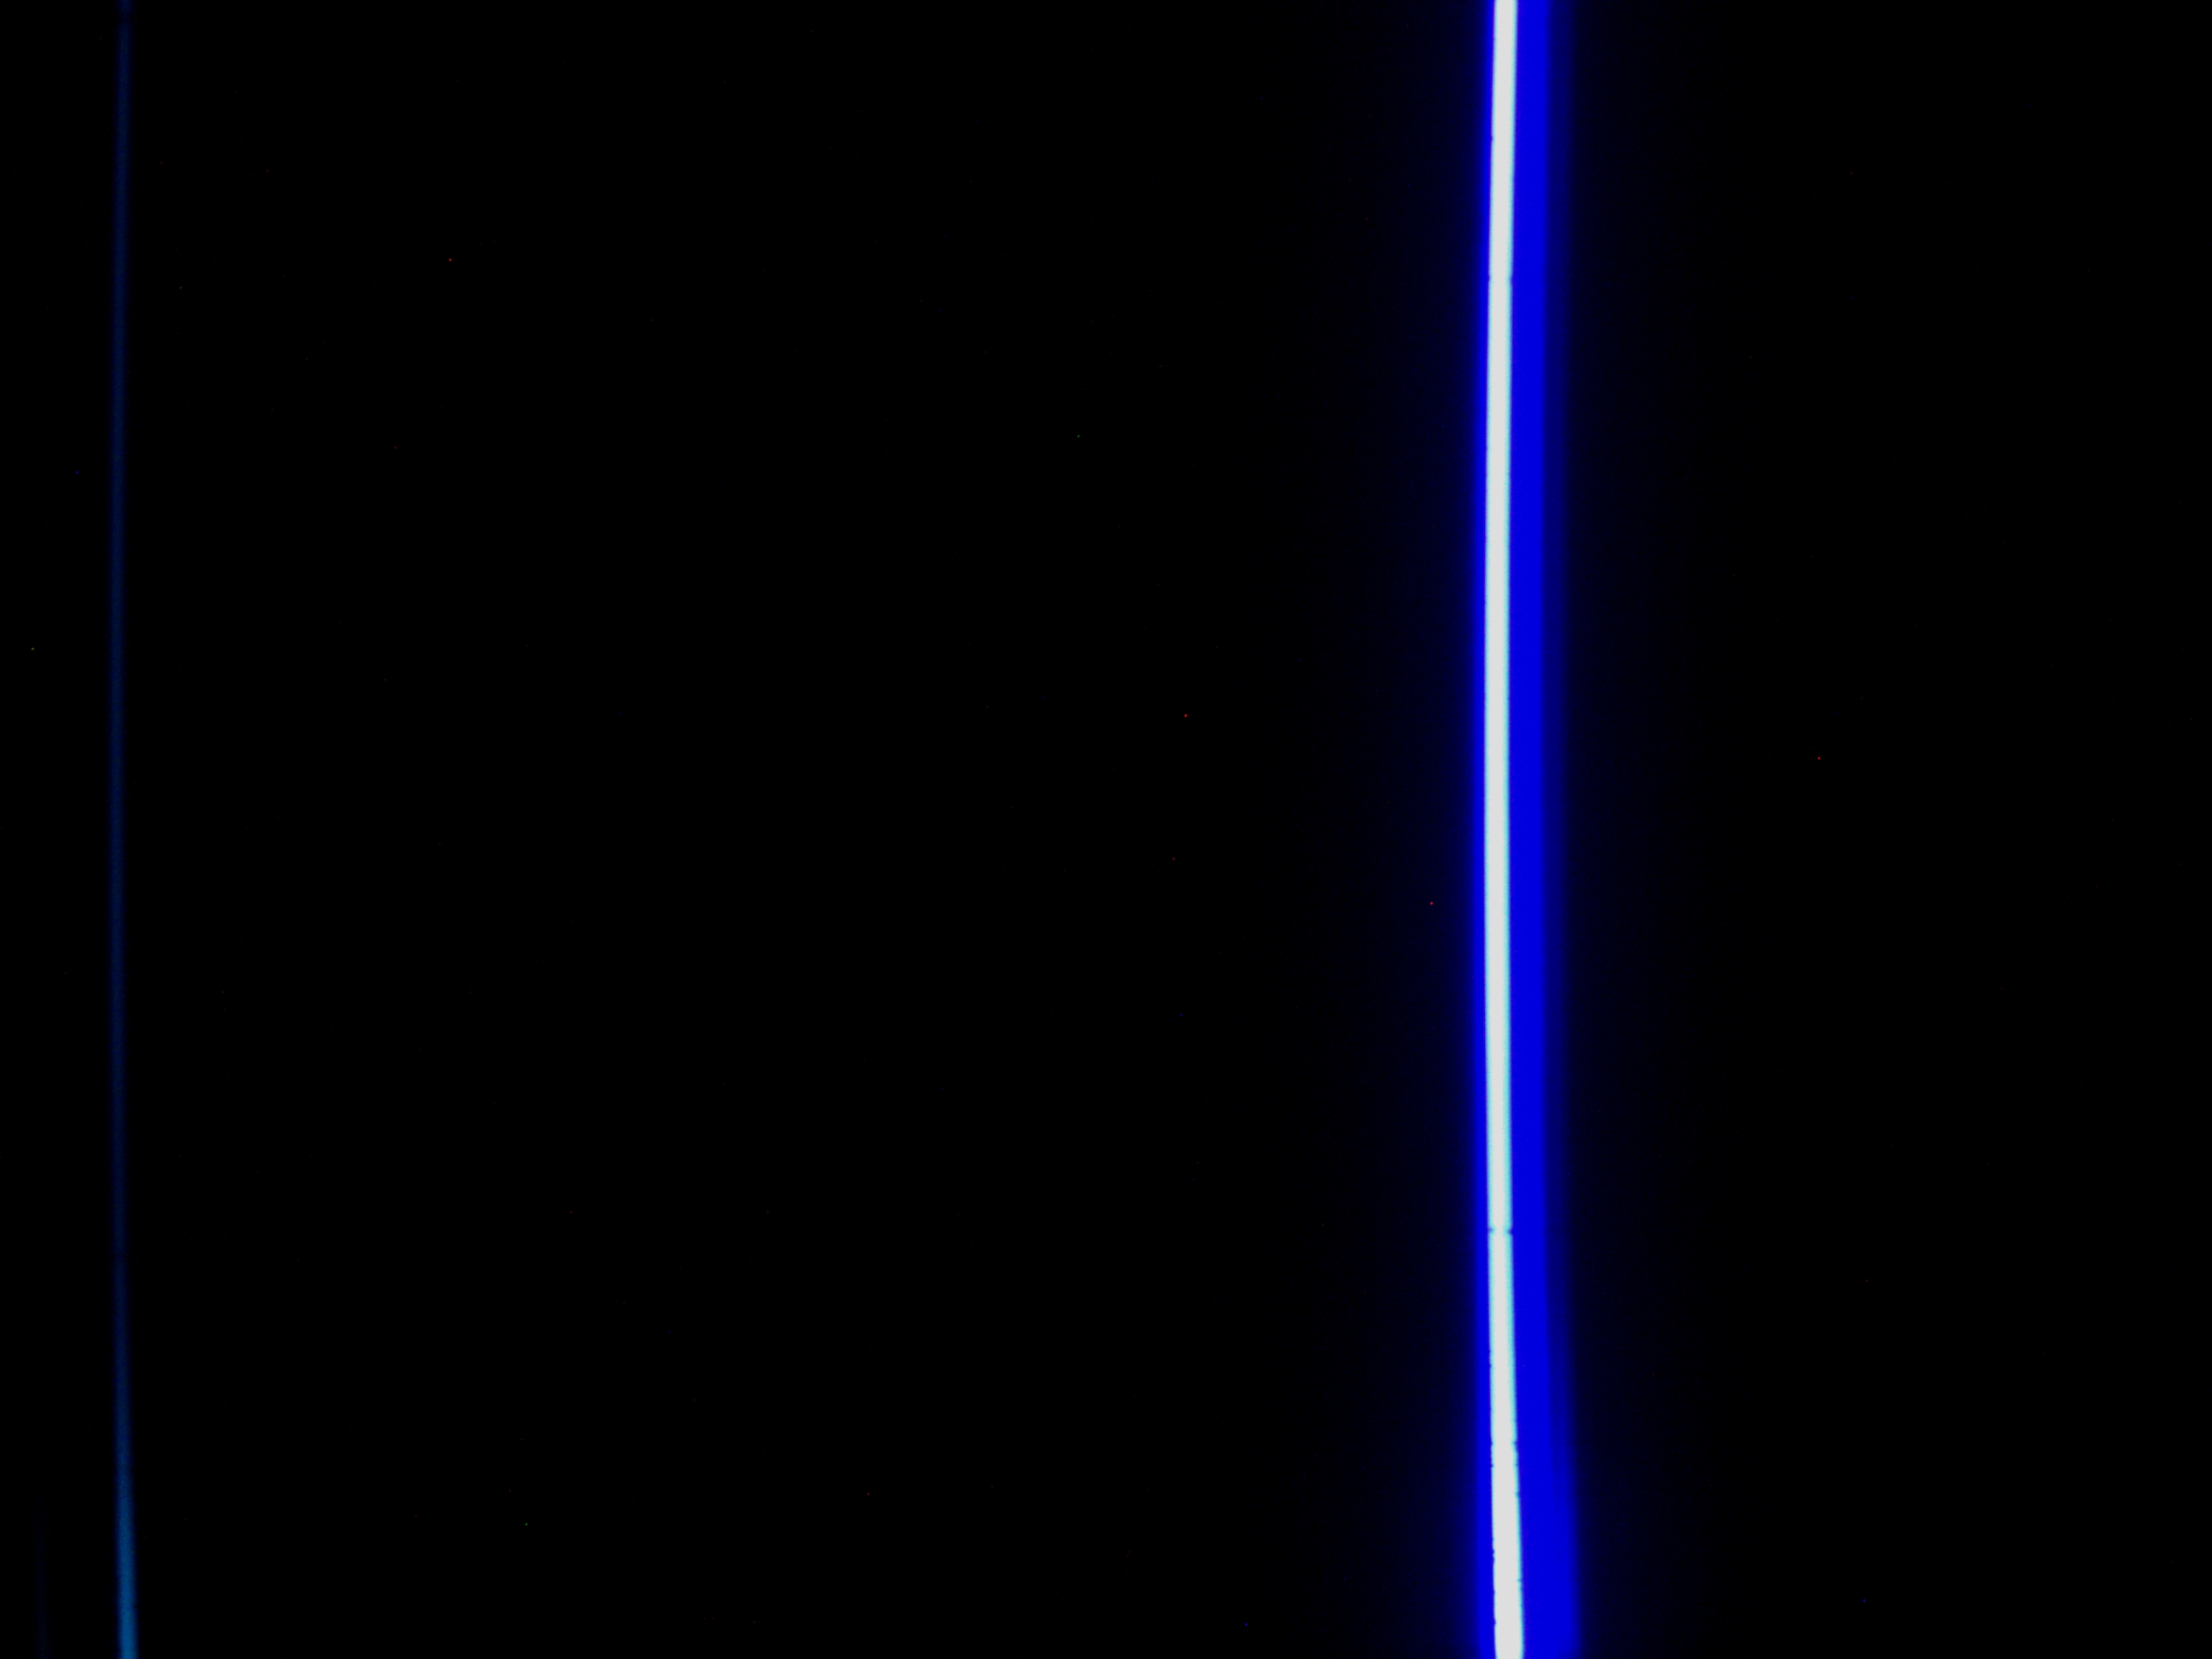
\includegraphics[scale=0.05]{3-2} \\\small{图2.2.3 汞灯右边位置}\centering
\end{minipage}

~\\
\begin{minipage}[c]{0.33\textwidth}
    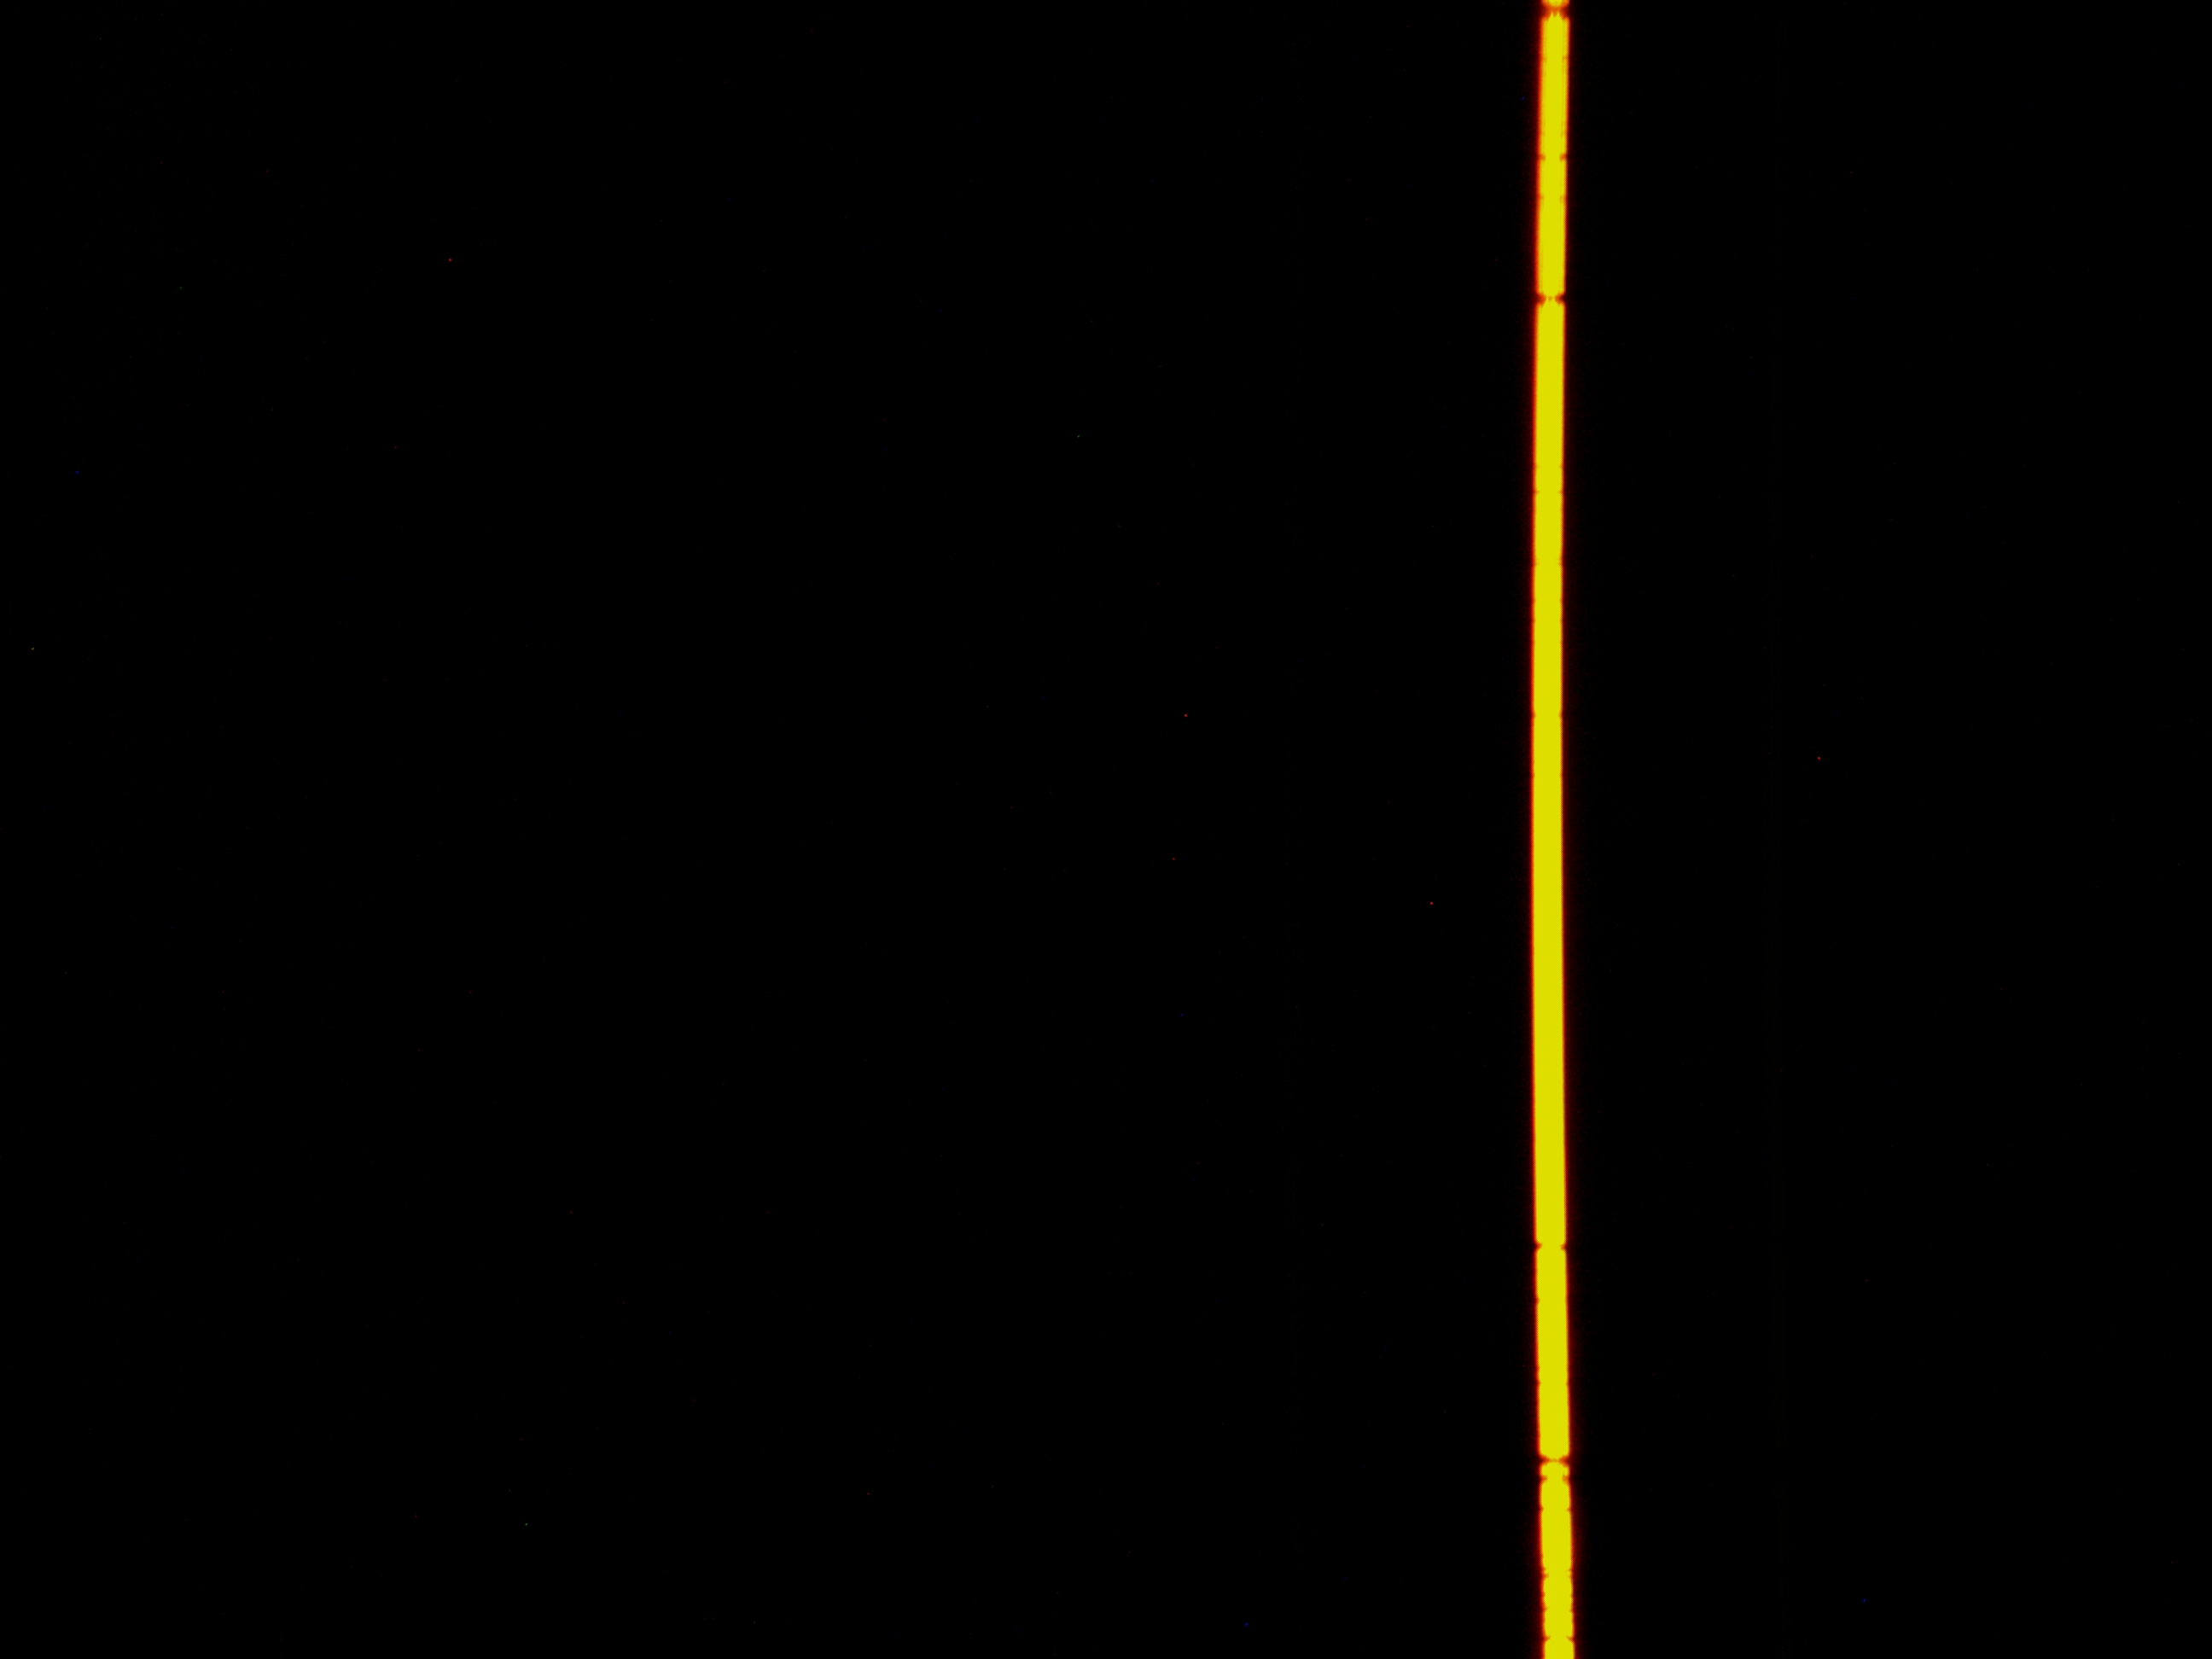
\includegraphics[scale=0.05]{1-3} \\\small{图2.3.1 钠灯左边位置}\centering
\end{minipage}
\begin{minipage}[c]{0.33\textwidth}
    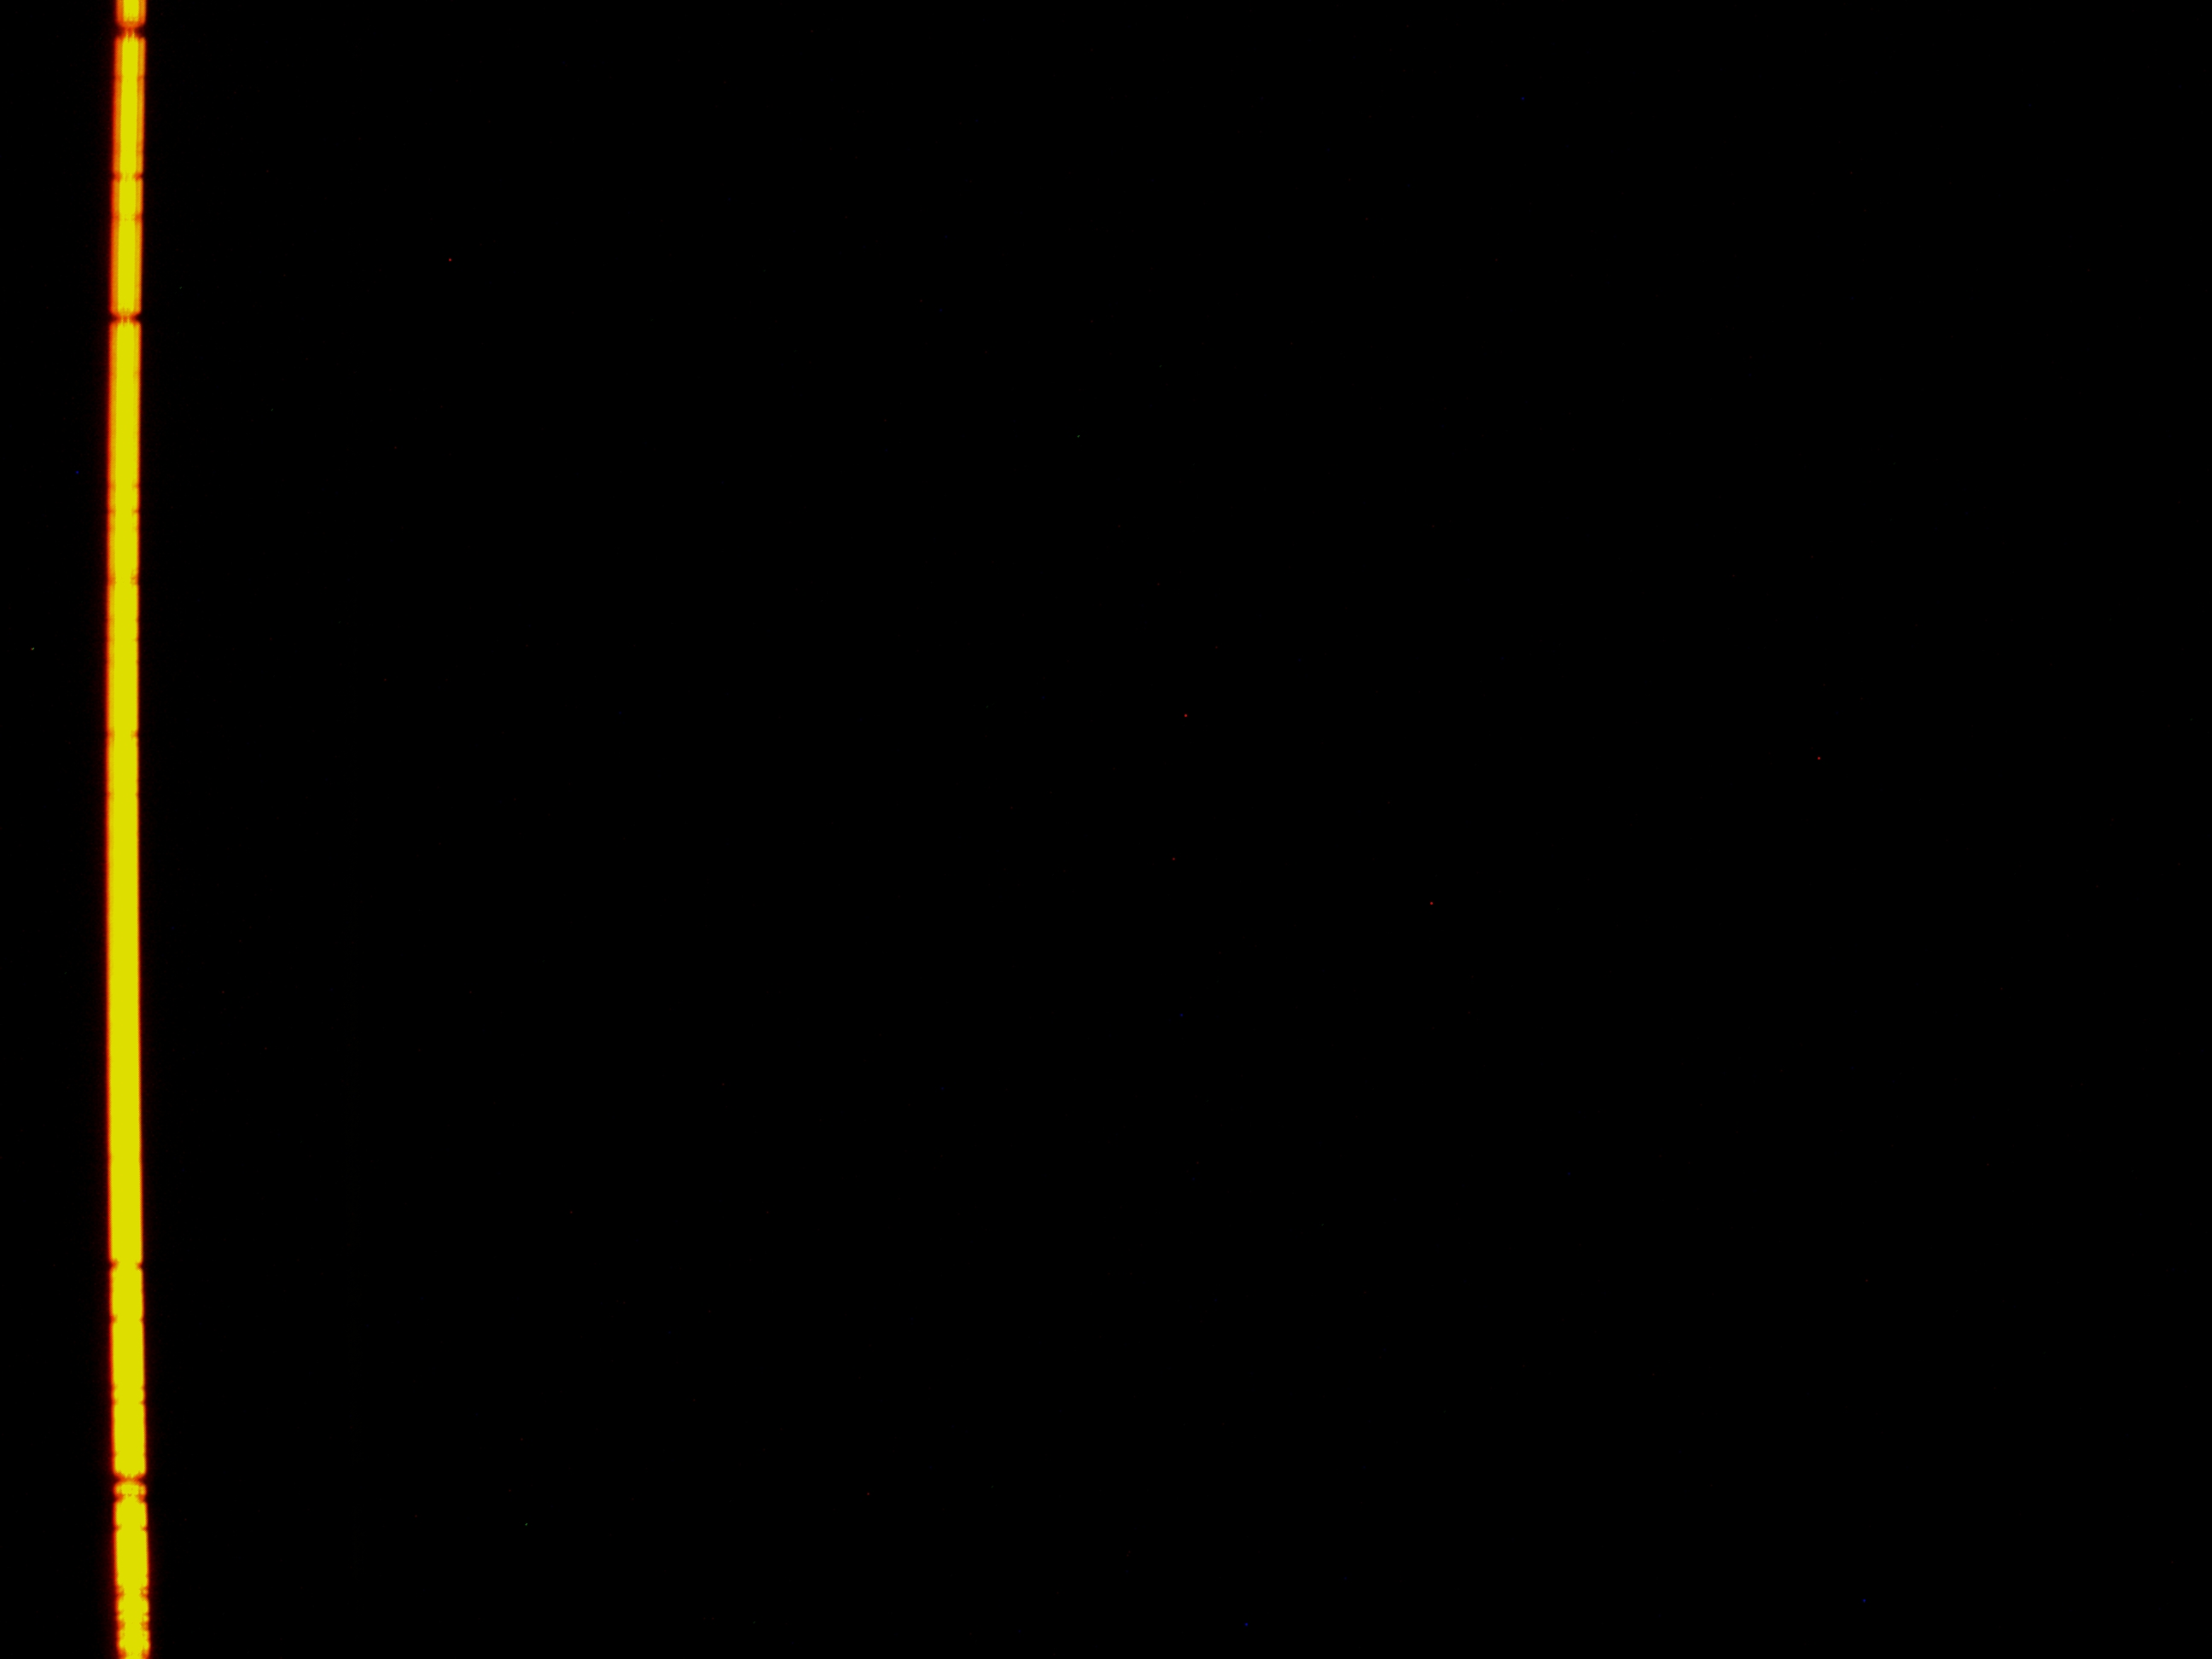
\includegraphics[scale=0.05]{2-3} \\\small{图2.3.2 钠灯中间位置}\centering
\end{minipage}
\begin{minipage}[c]{0.33\textwidth}
    
\includegraphics[scale=0.05]{3-3} \\\small{图2.3.3 钠灯右边位置}\centering
\end{minipage}

~\\

传统的数据处理方法为用PowerPoint等软件手动拼接谱线,保证氦谱相同的谱线重合,然后保持垂直方向对齐,拼接汞谱和钠谱。然后记录拼接后每条谱线的横向相对位置。但是这种方法受限于手动判断拼接,导致精度不高。本实验中使用基于VB,NET,WPF的摄谱处理程序进行处理。

下面是具体的操作步骤。

1.将图片导入计算机程序;

2.寻峰。使用极值法,程序比较每个像素点与左右像素点的亮度,最亮处即为谱线位置。通过不断调节参数“升降亮度容差”,使得识别所有谱线的同时,避免将杂点识别为谱线;

3.拼接。不断调节参数“色相容差”和“亮度容差”,将前一张图与后一张图谱线的色相和亮度匹配,以拼接成一张完整光谱;

4.插值。将作为参考谱线的氦灯波长输入,程序使用插值法,得到汞谱与钠谱的谱线波长。反转底色,得到下图:

~\\
\begin{minipage}[c]{1\textwidth}
    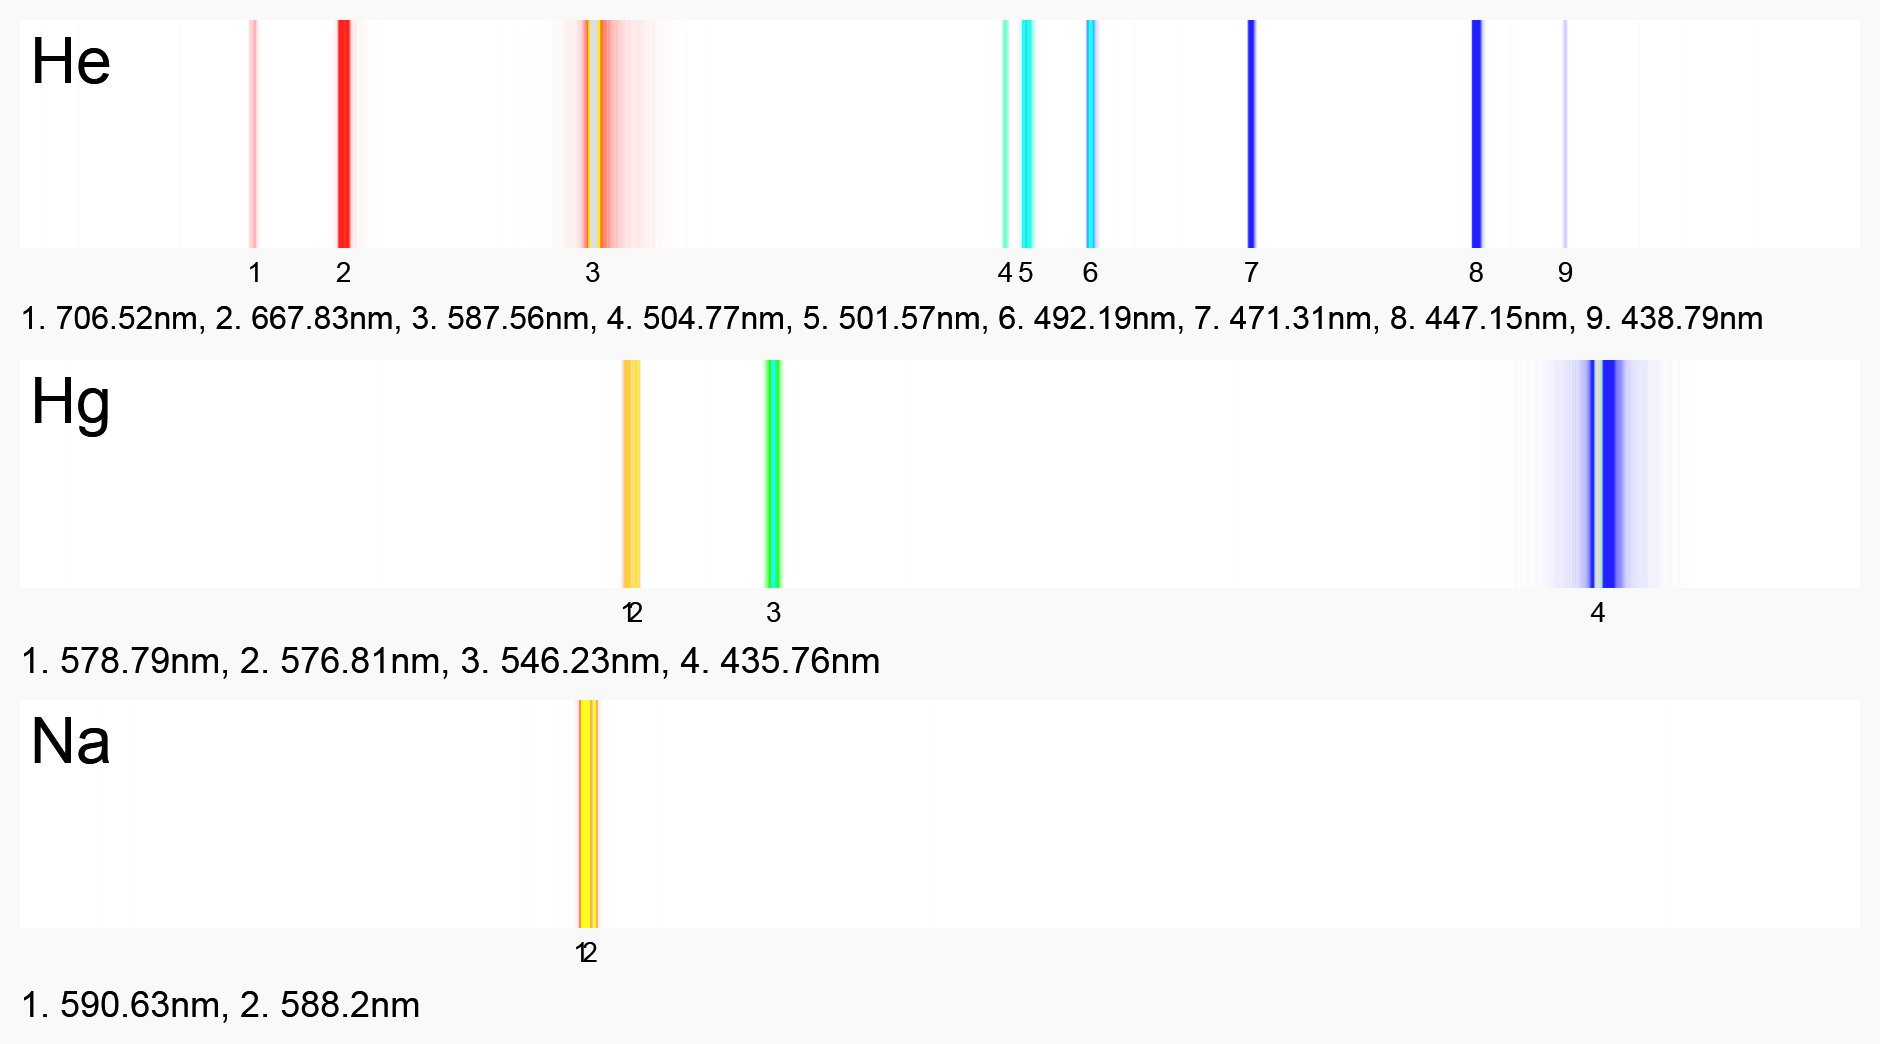
\includegraphics[scale=0.7]{white} \\\small{图3.处理结果}\centering
\end{minipage}

~\\
得到结果为

汞谱:黄(暗):578.79nm,576.81nm;绿:546.23nm;紫:435.76nm。

钠谱:黄:590.63nm,588.2nm。

(参考谱线:氦谱:红(暗):706.52nm,红:667.83nm,黄587.56nm,绿(暗):504.77nm,绿:501.57nm,蓝绿:492.19nm,蓝:471.31nm,紫:447.15nm,紫(暗):438.79nm)

\section*{第三部分 \qquad 误差分析}

查阅资料,标准值为:

汞谱:黄(暗):579.07nm,576.96nm,绿:546.07nm,天蓝(暗):491.60nm,紫:435.84nm。

钠谱:黄:589.00nm,589.59nm。

可以发现实验数据与标准值误差很小。汞谱中天蓝色暗线没有拍出,结合实验讲义及ppt中的参考图片(也没有天蓝色谱线),猜测可能是因为汞谱中紫色谱线过强,导致很难同时保证紫色谱线粗细合适与识别天蓝色暗线。

\section*{第四部分 \qquad 思考题}

\subsection*{1. 实验中影响光谱清晰度的调节机构有哪些?}

实验中影响光谱清晰度的调节机构有聚光透镜L到狭缝的距离,聚光透镜L的高度,光源到聚光透镜的距离,光源高度,狭缝大小,会聚透镜 $L_2$的角度,CCD到出光口之间的距离等。

\subsection*{2. 实验中, CCD 靶面的横向宽度小于光谱成像面的横向宽度, 实验中是如何完成的?}

光谱线使用三张图片分段拍摄,处理时将三幅图片拼接在一起成为一个整体。在拍摄不同光源的相同位置时保持CCD位置不变。

\subsection*{3. 本实验中,能否将光谱成像面的横向宽度做到小于或等于 CCD 的靶面横向宽度?如果能,怎么做?实际实验中未做,可能的原因是什么?}

光学元件有一定的最小焦距和成像能力限制。因此,要使光谱成像面的横向宽度小于或等于CCD的靶面横向宽度,需要采用以下方法:

1.使用具有更大底片的CCD。实现更广的成像范围,从而使CCD的靶面横向宽度更大。

2.增加光学系统的放大倍数。通过增加光学系统的放大倍数,从而使光谱成像面的横向宽度更小。

实际实验中未能将光谱成像面的横向宽度做到小于或等于CCD靶面横向宽度可能有以下原因:

1.实验所采用的光学元件的设计和性能限制,无法实现将光谱成像面的横向宽度缩小到目标值以下。

2.不将光谱成像面的横向宽度做到小于或等于CCD靶面横向宽度,对实验结果及误差的影响在可以接受的范围之内。

3.成本问题,无法使用更大底片的CCD。

\subsection*{4. 三棱镜可以作为分光元件的原因是什么?}
利用三棱镜对不同波长的光有不同折射率的性质来进行分光。折射率 $n$ 与光的波长$\lambda$有关。当一束白光或其它非单色光入射到棱镜时,由于折射率不同,不同波长的光具有不同的偏向角,从而出射光线方向不同。通常棱镜的折射率 $n$ 是随波长 $\lambda$ 负相关,所以可见光中紫光偏折最大,红光偏折最小。因此可以作为分光元件。

\section*{致谢}
\begin{center}
	感谢中国科学技术大学物理实验教学中心和田佳冉老师
\end{center}


\label{unknown}
\end{document}